\documentclass[10pt,a4paper]{article}
%%%%%%%%%%%%%%%%%%%%%%%%%%%%%%%%%%%%%%%%%%%%
%                 PACKAGES
%%%%%%%%%%%%%%%%%%%%%%%%%%%%%%%%%%%%%%%%%%%%

% LANGUAGE AND ENCODING
\usepackage[utf8]{inputenc}      % Direct UTF-8 character input
\usepackage[english]{babel}      % Language-specific hyphenation
\usepackage{xstring}

% CORE MATHEMATICS
\usepackage{amsmath}             % AMS math environments (align, gather, etc.)
\usepackage{amssymb}             % AMS math symbols
\usepackage{amsthm}              % Theorem environments
\usepackage{amsfonts}            % AMS fonts
\usepackage{mathtools}           % Extensions to amsmath
\usepackage{esint}               % Extended integral symbols
\usepackage{cancel}              % Diagonal cancellation in math
\usepackage{tcolorbox}           % Good boxes
\tcbuselibrary{most}

\usepackage{lmodern}
\usepackage{bm}                  % Bold math symbols (Greek, etc.)
\usepackage{mathrsfs}            % Ralph Smith's script font
\usepackage{tensor}              % Tensor index notation

% UNITS AND QUANTITIES
\usepackage{siunitx}             % Professional number and unit formatting
\NewCommandCopy\uqty\qty         % Save siunitx's \qty as \uqty
\usepackage{silence}
\WarningFilter{siunitx}{Detected the "physics" package}
\ExplSyntaxOn
\msg_redirect_name:nnn { siunitx } { physics-pkg } { none }
\ExplSyntaxOff

% TABLES AND BOXES
\usepackage{tabulary}            % Tables with automatic width adjustment
\usepackage{mdframed}            % Framed boxes with backgrounds
% \usepackage{chemformula}       % Alternative chemistry notation (commented)

% MATH TOOLS
\usepackage{centernot}           % Centered negation symbol
\usepackage{dcolumn}             % Decimal alignment in tables
\usepackage[shortlabels]{enumitem} % Customizable lists

% GRAPHICS AND FIGURES
\usepackage{graphicx}            % Include images
\usepackage{float}               % Force figure placement with [H]
\usepackage{tikz}                % Powerful diagram drawing
\usetikzlibrary{positioning,arrows,trees,3d,angles} % TikZ libraries
\usepackage{pgfplots}            % Scientific plots based on tikz
\pgfplotsset{compat=1.18}        % PGFPlots compatibility mode
\usepackage{subcaption}          % Subfigures (a), (b), etc.
\usepackage{caption}             % Customize caption formatting
\usepackage{booktabs}            % Professional tables with \toprule

% MULTI-COLUMN AND ARRAYS
\usepackage{multicol}            % Multi-column text layout
\usepackage{array}               % Enhanced table column types

% CHEMISTRY
\usepackage{chemfig}             % Draw molecular structures
\usepackage[version=4]{mhchem}   % Chemical equations in text (\ce{H2O})

% CIRCUITS
\usepackage{circuitikz}          % Circuit diagrams with tikz

% TEXT FORMATTING
\usepackage{blindtext}           % Lorem ipsum placeholder text
\usepackage{titlesec}            % Customize section headings
\usepackage{fancyhdr}            % Custom headers and footers
\usepackage{csquotes}            % Context-sensitive quotes

% HYPERLINKS
\usepackage[colorlinks=true, allcolors=blue]{hyperref} % Clickable links

% PAGE GEOMETRY
\usepackage[top=1.0in,bottom=1.0in,left=1.0in,right=1.0in,marginparwidth=1.75cm]{geometry}

% CODE LISTINGS
\usepackage{xcolor}              % Color definitions
\usepackage{listings}            % Code syntax highlighting
\usepackage{xparse}              % Robust command definitions
\usepackage{braket}              % Dirac bra-ket notation

% PHYSICS PACKAGES (LOADED LAST)
\usepackage[italicdiff]{physics} % Original physics package (d in italics)
\usepackage{physics2}            % Modern physics package
\usephysicsmodule{ab}            % Auto-braces module
\usephysicsmodule{ab.legacy}     % Legacy \abs, \norm, \eval
\usephysicsmodule{nabla.legacy}  % \grad, \div, \curl operators
\usephysicsmodule{op.legacy}     % Operators like \tr, \Re, \Im
\usephysicsmodule{diagmat, xmat} % Diagonal and special matrices
\usephysicsmodule{braket, ab.braket} % Dirac notation
\let\lpc\laplacian               % Alias for Laplacian

%%%%%%%%%%%%%%%%%%%%%%%%%%%%%%%%%%%%%%%%%%%%
%             NEW COMMANDS
%%%%%%%%%%%%%%%%%%%%%%%%%%%%%%%%%%%%%%%%%%%%

%%% MATH OPERATORS
\DeclareMathOperator{\sinc}{sinc}
\DeclareMathOperator{\sgn}{sgn}

%%% INVERSE TRIGONOMETRIC OPERATORS
\renewcommand{\asin}{\sin^{-1}}
\renewcommand{\acos}{\cos^{-1}}
\renewcommand{\atan}{\tan^{-1}}
\renewcommand{\acsc}{\csc^{-1}}
\renewcommand{\asec}{\sec^{-1}}
\renewcommand{\acot}{\cot^{-1}}

\newcommand{\asinh}{\sinh^{-1}}
\newcommand{\acosh}{\cosh^{-1}}
\newcommand{\atanh}{\tanh^{-1}}
\newcommand{\acsch}{\csch^{-1}}
\newcommand{\asech}{\sech^{-1}}
\newcommand{\acoth}{\coth^{-1}}
% \DeclareMathOperator{\arcsin}{arcsin}
% \DeclareMathOperator{\arccos}{arccos}
% \DeclareMathOperator{\arctan}{arctan}
% \DeclareMathOperator{\arccsc}{arccsc}
% \DeclareMathOperator{\arcsec}{arcsec}
% \DeclareMathOperator{\arccot}{arccot}
\DeclareMathOperator{\arsinh}{arsinh}
\DeclareMathOperator{\arcosh}{arcosh}
\DeclareMathOperator{\artanh}{artanh}
\DeclareMathOperator{\arcsch}{arcsch}
\DeclareMathOperator{\arsech}{arsech}
\DeclareMathOperator{\arcoth}{arcoth}

%%% NUMBER SETS
\newcommand{\R}{\mathbb{R}}          % Real numbers
\newcommand{\Z}{\mathbb{Z}}          % Integers
\newcommand{\Q}{\mathbb{Q}}          % Rational numbers
\newcommand{\C}{\mathbb{C}}          % Complex numbers
\newcommand{\N}{\mathbb{N}}          % Natural numbers
\newcommand{\K}{\mathbb{K}}          % Field R or C
\newcommand{\bb}[1]{\mathbb{#1}}     % Generic blackboard bold

%%% PARTIAL DIFFERENTIALS
\newcommand{\p}{\partial}            % Partial symbol

%%% VECTOR CALCULUS
\newcommand{\krondelta}[1]{\delta_{#1}}
\newcommand{\levicivita}[1]{\varepsilon_{#1}}
\newcommand{\ihat}{\vu*{\imath}}
\newcommand{\jhat}{\vu*{\jmath}}
\newcommand{\khat}{\vu*{k}}
\newcommand{\rhohat}{\vu*{\rho}}
\newcommand{\phihat}{\vu*{\phi}}
\newcommand{\thetahat}{\vu*{\theta}}
\newcommand{\rhat}{\vu*{r}}
\newcommand{\inv}{^{-1}}
\newcommand{\vell}{\boldsymbol{\ell}}

%%% DIFFERENTIALS AND TRANSFORMS
\newcommand{\laplace}[1]{\mathscr{L}\qty{#1}}
\newcommand{\invlaplace}[1]{\mathscr{L}^{-1}\qty{#1}}
\newcommand{\unitstep}[1]{\mathscr{U}\qty{#1}}
\newcommand{\intfty}{\int_{-\infty}^{+\infty}}

%%% PARENTHESES
\newcommand{\floor}[1]{\lfloor #1 \rfloor}
\newcommand{\ceiling}[1]{\lceil #1 \rceil}
\newcommand{\round}[1]{\lfloor #1 \rceil}
\newcommand{\nvec}[3]{\left\langle #1 , #2 , #3 \right\rangle}
\newcommand{\tline}[1]{\hrule \vspace{#1} \hrule}
\newcommand{\blank}[1]{\hspace*{#1}}

%%% TRANSFORM OPERATORS
\newcommand{\Laplace}{\mathscr{L}}
\newcommand{\Fourier}{\mathscr{F}}

%%% LOGICAL OPERATORS
\newcommand{\union}{\cup}
\newcommand{\intersect}{\cap}
\newcommand{\defined}{:=}

%%% COMPLEX ANALYSIS
\newcommand{\Arg}{\operatorname{Arg}}
\newcommand{\Hol}{\operatorname{Hol}}
\newcommand{\Log}{\operatorname{Log}}

%%% LINEAR ALGEBRA
\newcommand{\Span}[1]{\operatorname{span}\qty(#1)}
\newcommand{\Rank}[1]{\operatorname{rank}\qty(#1)}
\newcommand{\nullity}[1]{\operatorname{nullity}\qty(#1)}
\DeclareMathOperator{\image}{im}

%%% TOPOLOGY
\newcommand{\Id}{\operatorname{Id}}
\newcommand{\Image}[1]{\operatorname{Im}\qty(#1)}
\newcommand{\comp}{^{c}}
\newcommand{\Prob}[1]{\operatorname{Pr}\qty(#1)}
\newcommand{\du}{\mathrm{d}}
\newcommand{\topo}[1]{\mathcal{#1}}

%%% MISCELLANEOUS
\newcommand{\notimplies}{\centernot\implies}

\NewDocumentCommand{\dimu}{O{\mkern-3mu} m}{
\left[
#1
\left[#2\right]
#1
\right]
}

\newcommand{\id}{\operatorname{id}}
\newcommand{\contradiction}{\Rightarrow\!\Leftarrow}
\newcommand{\transition}[3]{{_{#2}\mathbf{#1}_{#3}}}
\newcommand{\barline}{\vspace{10pt}\hrule\vspace{10pt}}
\newcommand{\eqques}{\stackrel{?}{=}}
\newcommand{\Gammaf}[1]{\Gamma\qty(#1)}
\renewcommand\qedsymbol{$\square$}


%%%%%%%%%%%%%%%%%%%%%%%%%%%%%%%%%%%%%%%%%%%%
%       CUSTOM HEADER / SECTION STYLES
%%%%%%%%%%%%%%%%%%%%%%%%%%%%%%%%%%%%%%%%%%%%

\fancypagestyle{titleheader}{
  \fancyhead{}
  \fancyhead{\vspace{2cm}\tline{3pt}\fancyfoot[c]{\thepage}}
  \renewcommand{\headrulewidth}{0pt}
}
\newcommand{\titlebars}{
  \maketitle
  \tline{3pt}
  \thispagestyle{titleheader}
}

%%% CUSTOM SUBSUBSUBSECTION (4-LEVEL HEADINGS)
\titleclass{\subsubsubsection}{straight}[\subsection]
\newcounter{subsubsubsection}[subsubsection]
\renewcommand\thesubsubsubsection{\thesubsubsection.\arabic{subsubsubsection}}
\renewcommand\theparagraph{\thesubsubsubsection.\arabic{paragraph}}
\titleformat{\subsubsubsection}{\normalfont\normalsize\bfseries}{\thesubsubsubsection}{1em}{}
\titlespacing*{\subsubsubsection}{0pt}{3.25ex plus 1ex minus .2ex}{1.5ex plus .2ex}

\makeatletter
\renewcommand\paragraph{\@startsection{paragraph}{5}{\z@}{3.25ex \@plus1ex \@minus.2ex}{-1em}{\normalfont\normalsize\bfseries}}
\renewcommand\subparagraph{\@startsection{subparagraph}{6}{\parindent}{3.25ex \@plus1ex \@minus .2ex}{-1em}{\normalfont\normalsize\bfseries}}
\def\toclevel@subsubsubsection{4}
\def\toclevel@paragraph{5}
\def\toclevel@subparagraph{6}
\def\l@subsubsubsection{\@dottedtocline{4}{7em}{4em}}
\def\l@paragraph{\@dottedtocline{5}{10em}{5em}}
\def\l@subparagraph{\@dottedtocline{6}{14em}{6em}}
\makeatother
\setcounter{secnumdepth}{4}
\setcounter{tocdepth}{4}

%%% CUSTOM SECTION TITLE FONT SIZES
% \titleformat*{\section}{\LARGE\bfseries}
% \titleformat*{\subsection}{\Large\bfseries}
% \titleformat*{\subsubsection}{\large\bfseries}
% \setlength{\parskip}{10pt}

%%%%%%%%%%%%%%%%%%%%%%%%%%%%%%%%%%%%%%%%%%%%
%             ENVIRONMENTS
%%%%%%%%%%%%%%%%%%%%%%%%%%%%%%%%%%%%%%%%%%%%

\newenvironment{amatrix}[1]{%
  \left(
  \begin{array}{@{}*{#1}{c}|c@{}}}{
\end{array}\right)}

\newenvironment{abmatrix}[1]{%
  \left[
  \begin{array}{@{}*{#1}{c}|c@{}}}{
\end{array}\right]}


%%%%%%%%%%%%%%%%%%%%%%%%%%%%%%%%%%%%%%%%%%%%
%          THEOREM STYLES
%%%%%%%%%%%%%%%%%%%%%%%%%%%%%%%%%%%%%%%%%%%%

% \theoremstyle{definition}
% \newtheorem{theorem}{Theorem}[subsection]
% \newtheorem{corollary}{Corollary}[theorem]
% \newtheorem{lemma}[theorem]{Lemma}
% \newtheorem{definition}{Definition}[subsection]
% \newtheorem{example}{Example}[subsection]

% \theoremstyle{remark}
% \newtheorem*{remark}{Remark}
% \newtheorem*{solution}{Solution}
% \newtheorem*{note}{Note}

%%%%%%%%%%%%%%%%%%%%%%%%%%%%%%%%%%%%%%%%%%%%
%        CODE LISTING STYLE
%%%%%%%%%%%%%%%%%%%%%%%%%%%%%%%%%%%%%%%%%%%%


% ============================================
% PYTHON STYLE
% ============================================
\definecolor{vscodeBackground}{RGB}{255,255,255}
\definecolor{vscodeForeground}{RGB}{10,10,10}
\definecolor{vscodeKeyword}{RGB}{60,60,200}
\definecolor{vscodeString}{RGB}{230,0,0}
\definecolor{vscodeComment}{RGB}{0,100,0}
\definecolor{vscodeFunction}{RGB}{220,220,170}
\definecolor{vscodeOperator}{RGB}{212,212,212}
\definecolor{vscodeNumber}{RGB}{181,206,168}

\lstdefinestyle{vscodepython}{
    backgroundcolor=\color{vscodeBackground},
    basicstyle=\ttfamily\footnotesize\color{vscodeForeground},
    commentstyle=\color{vscodeComment},
    keywordstyle=\color{vscodeKeyword}\bfseries,
    stringstyle=\color{vscodeString},
    numberstyle=\tiny\color{vscodeForeground},
    identifierstyle=\color{vscodeForeground},
    morekeywords={True, False, None, and, as, assert, async, await, break, class,
        continue, def, del, elif, else, except, finally, for, from, global, if,
        import, in, is, lambda, nonlocal, not, or, pass, raise, return, try,
        while, with, yield},
    frame=single,
    rulecolor=\color{vscodeForeground},
    breaklines=true,
    numbers=left,
    numbersep=5pt,
    showstringspaces=false,
    tabsize=4,
    captionpos=b,
}

% ============================================
% C/C++ STYLE (FIXED)
% ============================================
\definecolor{vscodeType}{RGB}{0,150,200}
\definecolor{vscodePreprocessor}{RGB}{150,0,150}
\definecolor{vscodeFunction}{RGB}{180,100,0}
\definecolor{vscodeOperator}{RGB}{180,60,180}

\lstdefinestyle{vscodecpp}{
    backgroundcolor=\color{vscodeBackground},
    basicstyle=\ttfamily\scriptsize\color{vscodeForeground},
    commentstyle=\color{vscodeComment},
    stringstyle=\color{vscodeString},
    numberstyle=\tiny\color{vscodeForeground},
    identifierstyle=\color{vscodeForeground},
    %
    % Keywords (class 1)
    keywords={auto, break, case, catch, class, const, constexpr, continue,
        default, delete, do, else, enum, explicit, extern, false, final,
        for, friend, goto, if, inline, mutable, namespace, new, noexcept,
        nullptr, operator, override, private, protected, public, register,
        return, sizeof, static, static_assert, struct, switch, template,
        this, throw, true, try, typedef, typeid, typename, using, virtual,
        volatile, while},
    %
    % Types (class 2) – highlighted with emph
    emph={bool, char, char16_t, char32_t, double, float, int, long, short,
          signed, unsigned, void, wchar_t, size_t, ptrdiff_t},
    emphstyle={\color{vscodeType}\bfseries},
    %
    % Preprocessor (class 3)
    emph={[2]define, elif, else, endif, error, if, ifdef, ifndef, include,
          line, pragma, undef},
    emphstyle={[2]\color{vscodePreprocessor}\bfseries},
    %
    % Standard library functions (class 4)
    emph={[3]printf, scanf, fprintf, fscanf, sprintf, sscanf, getchar, putchar,
          gets, puts, fopen, fclose, fread, fwrite, malloc, calloc, realloc,
          free, exit, abort, assert, system, getenv, qsort, bsearch, memcpy,
          memset, memcmp, strlen, strcpy, strncpy, strcat, strncat, strcmp,
          strncmp, strstr, strtok, atoi, atof, atol, rand, srand, time, clock,
          pow, sqrt, exp, log, log10, sin, cos, tan, asin, acos, atan, atan2,
          fabs, floor, ceil, fmod, feof, ferror, clearerr, remove, rename,
          tmpfile, tmpnam, setbuf, setvbuf, rewind, fgetc, fputc, ungetc,
          fgets, fputs},
    emphstyle={[3]\color{vscodeFunction}\bfseries},
    %
    % C++ extra keywords (add to class 1)
    morekeywords={alignas, alignof, and, and_eq, bitand, bitor, compl,
        concept, const_cast, decltype, dynamic_cast, module, not, not_eq,
        or, or_eq, reinterpret_cast, requires, static_cast, xor, xor_eq},
    %
    % STL types and functions (add to class 4 via emph again)
    emph={[4]std, vector, map, set, string, array, deque, list, queue, stack,
          pair, tuple, unique_ptr, shared_ptr, weak_ptr, make_shared, make_unique,
          move, forward, function, bind, cout, cin, endl, cerr, clog,
          ifstream, ofstream, fstream, stringstream, istringstream, ostringstream,
          sort, find, transform, accumulate, for_each, copy, reverse, unique,
          remove, replace, swap, min, max, lower_bound, upper_bound, binary_search},
    emphstyle={[4]\color{vscodeFunction}\bfseries},
    %
    frame=single,
    rulecolor=\color{vscodeForeground},
    breaklines=true,
    numbers=left,
    numbersep=5pt,
    showstringspaces=false,
    tabsize=4,
    captionpos=b,
}

% ============================================
% SET DEFAULTS
% ============================================
\lstset{style=vscodepython, language=Python}


%% EMPHASIS BOX

\newtcolorbox{emphasis}{
  colback=white,        % White background
  colframe=black,       % Black border
  boxrule=0.5pt,        % Border thickness
  arc=0pt,              % Sharp corners (0pt = no rounding)
  left=6pt,             % Left padding
  right=6pt,            % Right padding
  top=6pt,              % Top padding
  bottom=6pt,           % Bottom padding
  boxsep=0pt,           % No extra separation
  before upper={
    \setlength{\abovedisplayskip}{0pt}
    \setlength{\abovedisplayshortskip}{0pt}
    \setlength{\belowdisplayskip}{0pt}
    \setlength{\belowdisplayshortskip}{0pt}
  }
}

%%%%%%%%%%%%%%%%%%%%%%%%%%%%%%%%%%%%%%%%%%%%
%             DOCUMENT SETTINGS
%%%%%%%%%%%%%%%%%%%%%%%%%%%%%%%%%%%%%%%%%%%%

\setlength{\parindent}{2em}
\setlength{\parskip}{5pt}
\newlength{\originalparindent}
\newlength{\originalparskip}
\AtBeginDocument{%
    \setlength{\originalparindent}{\parindent}%
    \setlength{\originalparskip}{\parskip}%
}
\numberwithin{equation}{section}

% SECTION TITLE FONT SIZES (move here from preset)
\titleformat*{\section}{\Large\bfseries}
\titleformat*{\subsection}{\large\bfseries}
\titleformat*{\subsubsection}{\large\bfseries}
\titleformat*{\subsubsubsection}{\bfseries}

% CUSTOM SECTION COMMANDS
\newcommand{\module}[1]{%
    \clearpage
    \refstepcounter{section}
    \vspace*{1cm}
    {\LARGE\bfseries\noindent Module \thesection\par}
    \vspace{0.5cm}
    {\noindent\Huge\bfseries #1\par}
    \vspace{2cm}
    \addcontentsline{toc}{section}{Module \thesection : #1}
}

\newcommand{\unitsec}[1]{%
    \clearpage
    \refstepcounter{section}
    \vspace*{1cm}
    {\LARGE\bfseries\noindent Unit \thesection\par}
    \vspace{0.5cm}
    {\noindent\huge\bfseries #1\par}
    \vspace{1.5cm}
    \addcontentsline{toc}{section}{Unit \thesection : #1}
}

\newcommand{\chaptersec}[2][\relax]{%
    \clearpage
    \refstepcounter{section}
    \vspace*{0.5cm}
    {\LARGE\bfseries\noindent Chapter \thesection\par}
    \vspace{0.5cm}
    {\noindent\huge\bfseries
        \ifx\relax#1\relax
            #2%
        \else
            #1%
        \fi
        \par
    }
    \vspace{1.5cm}
    \addcontentsline{toc}{section}{Chapter \thesection : #2}
}

%%% PROBLEM ENVIRONMENT (was in preset.tex, now here)
\newenvironment{problem}{%
    \hrule
    \vspace{5pt}
}{%
    \vspace{10pt}\hrule\vspace{10pt}
}

\newenvironment{solution_pset}{%
    \noindent\textbf{\Large Solution}\\[0.5cm]
}{%
    \newpage
}


%%% DEFINITION ENVIRONMENT
% Definition counter linked to section
\newcounter{definition}[section]
\renewcommand{\thedefinition}{\thesection.\arabic{definition}}

\newtcolorbox{definition}[2][]{%
    colback=white,
    colframe=black,
    boxrule=0.5pt,
    arc=0pt,
    left=6pt,
    right=6pt,
    top=6pt,
    bottom=6pt,
    fonttitle=\bfseries,
    title={%
        \stepcounter{definition}% Increment counter
        Definition \thedefinition{} : #2% Then display
    },
    #1
}

%%% EXAMPLE ENVIRONMENT
% Example counter linked to section
\newcounter{example}[section]
\renewcommand{\theexample}{\thesection.\arabic{example}}

\newtcolorbox{example}[2][]{%
    breakable,
    colback=white,
    colframe=blue,
    boxrule=0.5pt,
    arc=4pt,
    left=6pt,
    right=6pt,
    top=6pt,
    bottom=6pt,
    fonttitle=\bfseries,
    parbox=false,  % Don't use parbox mode
    before upper={%
        \setlength{\parindent}{\originalparindent}%
        \setlength{\parskip}{\originalparskip}%
        \noindent%
    },
    title={%
        \refstepcounter{example}%
        Example \theexample{} : #2%
    },
    #1
}

%%% THEOREM ENVIRONMENT
% Theorem counter linked to section
\newcounter{theorem}[section]
\renewcommand{\thetheorem}{\thesection.\arabic{theorem}}
\definecolor{darkred}{RGB}{139, 0, 0} 
\newenvironment{theorem}[2][]{%
    \refstepcounter{theorem}%
    \begin{tcolorbox}[
        colback=white,
        colframe=darkred,
        coltitle=white,
        colbacktitle=darkred,
        boxrule=0.5pt,
        arc=0pt,
        left=6pt,
        right=6pt,
        top=6pt,
        bottom=6pt,
        fonttitle=\bfseries,
        title={Theorem \thetheorem{} : #2},
        #1
    ]
}{%
    \end{tcolorbox}%
}

%%% NOTE ENVIRONMENT
\definecolor{darkgray}{RGB}{100, 100, 100}

\newtcolorbox{note}{%
    colback=white,
    colframe=darkgray,
    boxrule=0.5pt,
    arc=0pt,
    left=6pt,
    right=6pt,
    top=6pt,
    bottom=6pt,
    before upper={%
        \noindent{\textit{Note : }}\par\vspace{1em}%
    }
}

%%% REMARK ENVIRONMENT
\newtcolorbox{remark}{%
    colback=white,
    colframe=darkgray,
    boxrule=0.5pt,
    arc=0pt,
    left=6pt,
    right=6pt,
    top=6pt,
    bottom=6pt,
    before upper={%
        \noindent\textbf{\textit{Remark : }}\par\vspace{1em}%
    }
}


\newcommand{\mbh}{M_\text{BH}}
\begin{document}
	\begin{center}
	  {\Large
		\hrule\vspace{3pt}\hrule\vspace{0.5em}
		\textsc{Undergraduate Thesis Report 1}\vspace{1em}
		\hrule\vspace{1em}
		\textbf{
		  The Mass Fallback Rate and Light Intensity Curve\\
		  generated by a Tidal Disruption Event on a\\
		  Constant Density Star\\[0.5cm]
		}
	  }
	  {\large
		Vercil Juan\\[1em]
		September 10, 2026\vspace{1em}
		\hrule\vspace{3pt}
		\hrule\vspace{0.5cm}
	  }
	\end{center}

	\section{Introduction}
		Following the work of O\~na et al.\cite{Ona2026}, we analyze the effect of Tidal 
		Disruption Events (TDEs) on the mass fallback rate of the disrupted 
		stellar material $\dot M$, as well as the characteristic luminosity curve
		$L$. In this work, we hope to recover the canonical result $\dot M \propto T^{-5/3}$
		fallback rate established by Rees\cite{Rees1988} and Phinney\cite{Phinney1989}, as well as some interesting results under the assumption that the 
		star is homogeneous, i.e., constant density.   

		%% algorithm, stellar part, blackhole part dM/dT = dM / dE x dE / dT

		A TDE occurs when a star strays too close to a supermassive black hole and is torn
		apart by tidal forces, flinging its debris in to a range of orbits. The general
		procedure to determine the mass fallback rate rests on the chain rule
		\begin{equation}
			\label{eq:fallbackrate}
			\dv{M}{T} = \dv{M}{E} \dv{E}{T},
		\end{equation}
		which factorizes the problem into two parts; a \textit{stellar part} and an \textit{black hole part}. 
		The stellar part determines how the star's mass is distributed across binding energies, which
		depends on the star's internal density profile. This density profile is usually treated as
		polytropic, however in this work we take it to be isotropic and homogeneous. The black hole part determines 
		how each debris parcel's orbital energy return over time, via Kepler's third law. Multiplying 
		the two returns the mass fallback rate, and since a fraction of the infalling debris' energy
		is radiated as it circularizes and accreets, this in turn produces an observable luminosity curve 
		\begin{equation}
			\label{eq:luminositycurve}
			L = \eta \dot M c^2
		\end{equation}
		where $\eta$ is the radiative efficiency of the blackhole, i.e., the fraction of the infalling 
		rest-mass energy that escapes as radiation, $\dot M c^2$ being the rest-mass energy flux of the fallback debris.
		In this work, we take a different but similar approach to arrive with $\dot M$ and $L$.

	\section{Disruption Dynamics}
		As a starting point, we consider a singular Schwarzchild blackhole with mass $M_\text{BH}$.
		We don't consider other effects such as galactic gravitational potential or other extrinsic effects as of yet. 
		The entire derivation will be purely Newtonian in nature.
		This is the simplest possible case, being a nontorating, spherically symmetric system. 
		At far distances $r$, the relativistic effects are negligible, and the entire system can
		be approximated by Newtonian dynamics. In this case, the black hole can be approximated as a point mass.
		This has a typical radial inverse gravitational potential.
		\begin{equation}
			\label{eq:potentialbh}
			\Phi_\text{BH} = - \frac{GM_\text{BH}}{r} 
		\end{equation}

		From here on, we just call it $\Phi$. Now, we specify the encounter. We consider a star, of mass $M_\star$, entering
		at a typical assumed parabolic trajectory, i.e., the characteristic orbital energy $E = 0$.
		We specify it so that the trajectory touches the tidal disruption radius, $R_t$, precisely.
		That is, it has a penetration factor $\delta$ of $1$.
		\begin{equation}
			\label{eq:penetrationfactor}
			\delta = \frac{R_t}{R_p} 
		\end{equation}
		where $R_p$ is the periapsis (called peribothron for blackholes). The system is sketched in Figure \ref{fig:TDE-approach}
		\begin{figure}[h]
			\centering
			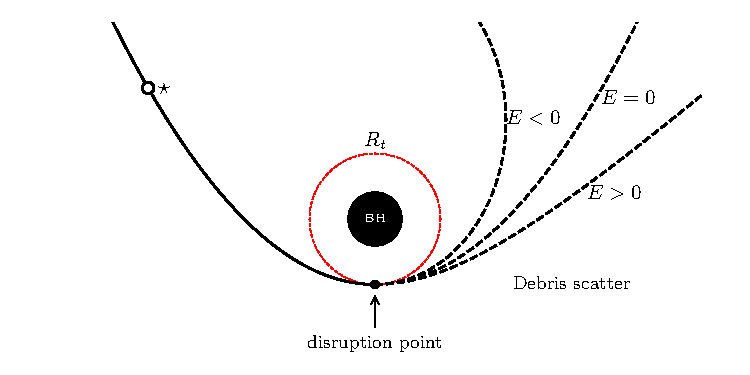
\includegraphics[width=5in, height = 2.5in]{images/approach.pdf}
			\caption{A star approaching a black hole at $R_t$}
			\label{fig:TDE-approach}
		\end{figure}

		Tidal disruption occurs when the tidal force exceeds the star's self gravity, i.e.,
		\begin{equation}
			\label{eq:tidal_disruption}
			\dv{\Phi(r - R_\star)}{r} - \dv{\Phi(r + R_\star)}{r} = \frac{GM_\star}{R_\star^2}
		\end{equation}
		Solving for $r$ gives $R_t$. For a typical Newtonian tidal radius, and when $R_\star \ll r$, this
		can be approximated by
		\begin{equation}
			\label{eq:tidalradius}
			R_t = R_\star \pqty{
				\frac{4M_\text{BH}}{M_\star} 
			}^{1/3}
		\end{equation}
		This is classically known as the Roche Limit (up to a factor of unity).
		The precise derivation is found in the \hyperref[appendices:a]{appendices}.

		Before the disruption, the center of mass of the star has energy
		\[
			E_\star = 0
		\]
		However, upon disruption, different parts of the star, depending on the distance from the blackhole, are imparted with different
		energies. This is expressed as 
		\begin{equation}
			\label{eq:Delta-E}
			\Delta E \simeq \pqty{\dv{\Phi}{r}}_{R_p} R_\star 
		\end{equation}

		For an initial approximation, $\dv*{\Phi}{r}$ is
		\[
			\dv{\Phi}{r} = \frac{G M_\text{BH}}{r^2}  
		\]
		therefore,
		\[
			\Delta E \simeq \frac{G M_\text{BH}}{R_p^2}  R_\star 
		\]

		After disruption, parts of the star acquire orbital energy $E\geq0$, which means it is 
		unbound, and $E<0$, which means it is bound. For this, we assume the ``frozen-in''
		approximation, where we assume that each part of the star instantaneously acquire
		the orbital energy at the point of disruption, and evolves ballistically over time. 

		Now, we imagine ``slicing'' the star in the direction perpendicular to the direction
		of the blackhole. Let $\Delta r$ be the distance of the slice from the center of the star,
		where $\Delta r > 0$ is towards the blackhole, and $\Delta r < 0$ is away (Fig. \ref{fig:star-slices}). 

		\begin{figure}[h]
			\centering
			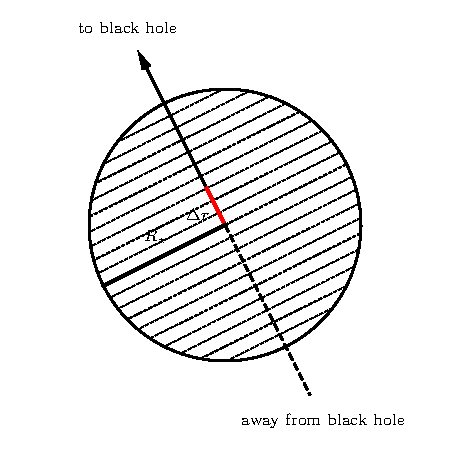
\includegraphics[width=3in]{images/slices.pdf}
			\caption{``Slicing'' the star to get the energy imparted}
			\label{fig:star-slices}
		\end{figure}
		
		From Lodato\cite{Lodato2009}, we adapt a dimensionless parameter $\xi$ such that
		\begin{equation}
			\label{eq:xidef}
			\xi = \frac{\Delta r}{R_\star} 
		\end{equation}
		The orbital energy of the star is then approximately linear in its profile
		\[
			E(\Delta r) \simeq - \frac{G\mbh}{R_p^2}\Delta r 
		\]

		We can then express $E$ in terms of $\xi$. 
		\[
			E \xi = -\Delta E\quad \implies\quad E(\xi) = -\Delta E \xi
		\]
		Equivalently,
		\[
			\xi = - \frac{E}{\Delta E} 
		\]
		
		The near side of the star has $\xi \geq 0$, thus $E \leq 0$ (bound), and the far side has $\xi < 0$, therefore $E > 0$ (unbound).

		So for the accretion curve, we only really care about
		\[
			0 < \xi \leq 1
		\]
	\section{Stellar Structure}
		Now, we need to know how much mass has each energy, i.e., we need to find $\displaystyle \dv{M}{E} $.

		Because $E = -\Delta E \xi$, then $\displaystyle \dv{E}{\xi}= -\Delta E$. Therefore,
		\[
			\dv{M}{E} = -\frac{1}{\Delta E} \dv{M}{\xi}
		\]
		To find $\dv*{M}{\xi}$, we need to consider how much mass is in each slice of the star. The 
		mass element is
		\begin{equation}
			\label{eq:mass-element}
			\dd{M} = 2\pi \dd{(\Delta r)} \int_{\Delta r}^{R_\star} \rho(r) r \dd{r}
		\end{equation}
		where $r$ is the radius of each slice from the center of the star (derivation at the Appendices). From (\ref{eq:mass-element}), we 
		can find the mass per each slice.
		\[
			\dv{M}{\Delta r} = 2\pi  
			\int_{\Delta r}^{R_\star} \rho(r) r \dd{r}
		\]
		For a dimensionless form, we can consider that since $\xi = \dfrac{\Delta r}{R_\star}$, we have $r = R_\star \xi'$, thus
		\[
			\dv{M}{\xi} = 2\pi R_\star^3 \int_\xi^1 \rho(R_\star \xi') \xi' \dd{\xi'}
		\]
		From the work of O\~na et al, they consider a polytropic star, where the density profile
		is spherically symmetric, $\rho(r)$, and can be solved by the Lane-Emden equation\cite{Seidov2001}
		\begin{equation}
			\label{eq:lane-emden}
			\frac{1}{\xi^2} \dv{}{\xi}\pqty{
				\xi^2 \dv{\theta}{\xi} 
			} = - \theta^n
		\end{equation}
		Where $\theta$ is a dimensionless density, and $\xi$ is a dimensionless radius. 
		In the work, they use a polytropic index of $n=3$, which corresponds to solar-type main 
		sequence stars. However, for the case of the current work, we consider a constant density
		star, i.e., the polytropic index is $n=0$. The Lane-Emden equation then reduces to 
		\[
			\frac{1}{\xi^2} \dv{}{\xi}\pqty{
				\xi^2 \dv{\theta}{\xi} 
			} = -1 .
		\]
		With the boundary conditions $\theta(0)=1$ and $\theta'=0$, the solution is simply
		\[
			\theta(\xi) = 1 - \frac{\xi^2}{6} 
		\]	
		For $\theta = 0$, we find the radius of the star. It turns out to be $R_\star = a\sqrt{6}$, where $a$ is the radial scale length. That 
		isn't really the point here, the point is that we now find that the star has a
		density profile of
		\begin{equation}
			\label{eq:homogenous-density}
			\rho(r) = \begin{cases}
				\rho_0, & 0\leq r \leq R_\star\\
				0, & r > R_\star
			\end{cases}
		\end{equation}
		where $\rho_0$ is the average density of the star. This density profile makes it possible
		to solve the stellar part of the procedure to be completely analytic. That is,
		\begin{align}
			\dv{M}{\Delta r} &=
			2\pi \int_{\Delta r}^{R_\star} \rho_0 r \dd{r}\notag\\
							 &= 2\pi\rho_0 \int_{\Delta r}^{R_\star} r \dd{r}\notag\\
							 &= 2\pi\rho_0 \eval{\frac{r^2}{2}}^{R_\star}_{\Delta r}\notag\\
							 &= 2\pi\rho_0 \pqty{\frac{R_\star^2}{2}- \frac{\Delta r^2}{2}}\notag\\
							 &= \pi\rho_0 \pqty{R_\star^2 - \Delta r^2}
		\end{align}
		Equivalently, in dimensionless form,
		\begin{align}
			\dv{M}{\xi}
			&=
			2\pi\rho_0 R_\star^3 \int_\xi^1 \xi' \dd{\xi'}\notag\\
			&= 2\pi\rho_0 R_\star^3 \eval{\frac{\xi'^2}{2}}^{1}_{\xi}\notag\\
			&= 2\pi\rho_0 R_\star^3 \pqty{ \frac{1}{2} - \frac{\xi^2}{2}}\notag\\
			&= \pi\rho_0 R_\star^3 \pqty{1 - \xi^2}
			\label{eq:dmdxi}
		\end{align}

	\section{Fallback Dynamics}
		For the black hole orbital dynamics, we proceed with the following. Each
		band of debris has original specific orbital energy $E= 0$. However, post-disruption, they each
		receive different energies. For a keplerian orbit, the specific orbital energy is
		\begin{equation}
			\label{eq:kepler-energy}
			E = -\frac{G\mbh}{2a} 
		\end{equation}
		where $a$ is the semi-major axis of the orbit. We can solve for it, and we find that
		\[
			a = 
			-\frac{G\mbh}{2E} 
		\]
		Kepler's third law gives the period of the orbit
		\[
			T = 2\pi \sqrt{\frac{a^3}{G\mbh}}
		\]
		Substituting $a$, we have
		\begin{align*}
			T
			&= 2\pi \sqrt{
				\frac{1}{G\mbh}
				\pqty{
					-\frac{G\mbh}{2E} 
				}^3
			}\\
			&= 2\pi G\mbh (-2E)^{-3/2}
		\end{align*}
		Since $E = -\Delta E \xi$, we get 
		\[
			T(\xi) = 
			2\pi G\mbh (-2\Delta E \xi)^{-3/2}
		\]
		
		We want the amount of material returning to $R_p$ at a particular time $T$ after the disruption, so we 
		invert the function.
		\begin{equation}
			\label{eq:xi-t}
			\xi(T) = \frac{1}{2\Delta E} \pqty{
				\frac{2\pi G\mbh}{T} 
			}^{2/3}
		\end{equation}

		At time $T$, the returning debris are those which have orbital period $T$. Therefore, we have
		\begin{equation}
			\label{eq:massfallbackxi}
			\dv{M}{T} = \dv{M}{\xi} \dv{\xi}{T}   
		\end{equation}
		Notice that this is the same form as (\ref{eq:fallbackrate}), but we swapped the energy $E$ to the dimensionless parameter $\xi$, i.e.,
		\[
			\dv{M}{T} = {
				\pqty{
					- \frac{1}{\Delta E} \dv{M}{E} 
				}
				\pqty{
					-\Delta E \dv{E}{T} 
				}
			} 
		\]
		
		Moving forward, we find that
		\begin{equation}
			\label{eq:dxidt}
			\dv{\xi}{T} 
			=
			-\frac{(2\pi G\mbh)^{2/3}}{3\Delta E} T^{-5/3} 
		\end{equation}
		Multiplying this with (\ref{eq:dmdxi}), we find that
		\begin{equation}
			\label{eq:dmdt}
			\dv{M}{\xi} \dv{\xi}{T}   
			= 
			-\pi\rho_0 R_\star^3 (1- \xi^2)  
			\frac{(2\pi G\mbh)^{2/3}}{3\Delta E} T^{-5/3} 
		\end{equation}
		Since $\rho_0 =\dfrac{3M_\star}{4\pi R_\star^3}$, then $\dfrac{\pi \rho_0 R_\star^3}{3} = \dfrac{M_\star}{4}$. Hence
		\[
			\dv{M}{T} = 
			\frac{M_\star (2\pi G\mbh)^{2/3}}{4\Delta E}
			(1-\xi^2) T^{-5/3}
		\]
		Expanding $\xi(T)$ from (\ref{eq:xi-t}), we have
		\[
			\dot{M} =  
			\frac{M_\star (2\pi G\mbh)^{2/3}}{4\Delta E}
			\pqty{1-
				\frac{1}{4\Delta E^2} \pqty{
					\frac{2\pi G\mbh}{T} 
				}^{4/3}
			}
			T^{-5/3}
		\]
		Simplifying this, we have the explicit expression for $\dot{M}$
		\begin{equation}
			\label{eq:mdot}
			\dot{M} 
			= 
			\frac{
				M_\star (2\pi G \mbh)^{2/3}
			}{4\Delta E} T^{-5/3}
			-
			\frac{
				M_\star (2\pi G \mbh)^2
			}{16 \Delta E^3} T^{-3}
		\end{equation}
		
		We can further expand $\Delta E$, but this is simply a constant independent of time, so I elected not to do so.
		Hence, we have derived the mass fallback rate for a constant density star (for the appropriate assumptions of approach specific orbital energy $E_\star=0$ and penetration factor $\delta = 1$). 
		However, at this point we indeed recover the canonical $\dot M \propto T^{-5/3}$ result, as well as a following $T^{-3}$ term.

		To find the light curve generated
		by this fallback rate, we simply multiply it by $\eta c^2$. The value of $\eta$ is approximately $\eta\approx 0.1$ 
		for a Schwarzschild black hole\cite{Noble2011}. The expression for the light curve is then
		\begin{equation}
			\label{eq:light-curve}
			L
			=
			\eta c^2
			\pqty{
				\frac{
					M_\star (2\pi G \mbh)^{2/3}
				}{4\Delta E} T^{-5/3}
				-
				\frac{
					M_\star (2\pi G \mbh)^2
				}{16 \Delta E^3} T^{-3}
			}
		\end{equation}
	\section{Fallback rate and Light curve plots}

		\begin{figure}[h]
			\centering
			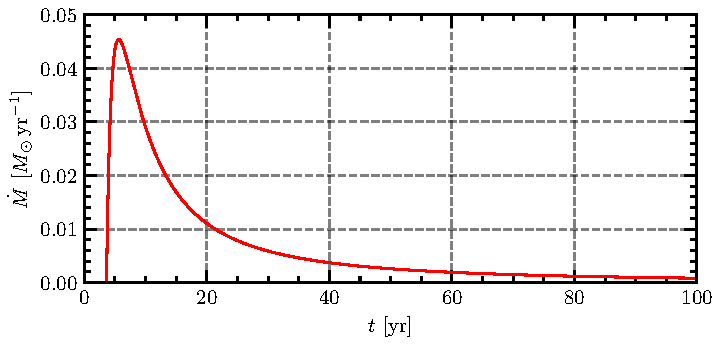
\includegraphics[width=5in]{images/mdot.pdf}
			\caption{Mass fallback rate of a solar-mass star disrupted by a $10^7 M_\odot$ black hole.}
			\label{fig:mdot}
		\end{figure}

		Figure \ref{fig:mdot} shows the mass fallback rate of a $1 M_\odot$ star disrupted by a 
		supermassive black hole with mass $10^7 M_\odot$, assuming a parabolic center-of-mass
		orbit with $E_\star=0$ and a penetration factor of $\delta=1$. The time $t$ denotes the
		elapsed time since the disruption, measured in years. At early times, approximately $0-5$ 
		years after disruption, the fallback rate initially increases as the negative $T^{-3}$ term
		dominates the expression for $\dot{M}$. The fallback rate subsequently reaches a maximum,
		after which it decreases as the $T^{-5/3}$ term becomes dominant at late times. Thus, the 
		long-time behavior approaches the canonical power-law dependence $\dot{M}\propto T^{-5/3}$.

		\begin{figure}[h]
			\centering
			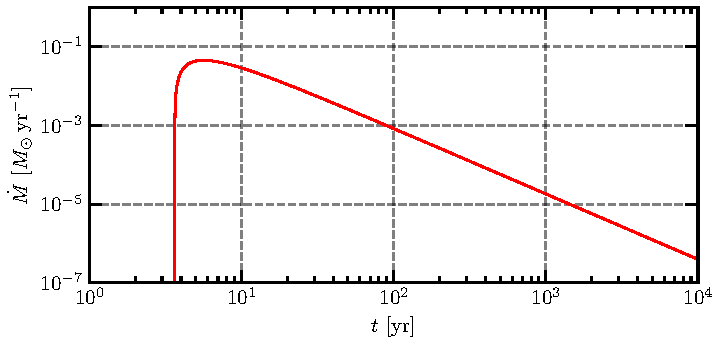
\includegraphics[width=5in]{images/mdot-log.pdf}
			\caption{Mass fallback rate of the same tidal disruption event as in Figure \ref{fig:mdot}, shown on a log-log scale.}
			\label{fig:mdot-log}
		\end{figure}

		Figure \ref{fig:mdot-log} shows the same event plotted on a log-log scale. The late-time
		fallback follows an approximately linear trend on the log-log plot, corresponding to the
		power-law dependence $\dot{M}\propto T^{-5/3}$. This asymptotic behavior becomes increasingly
		apparent at longer times as the $T^{-3}$ contribution becomes negligible compared with the 
		$T^{-5/3}$ contribution.

		\begin{figure}[h]
			\centering
			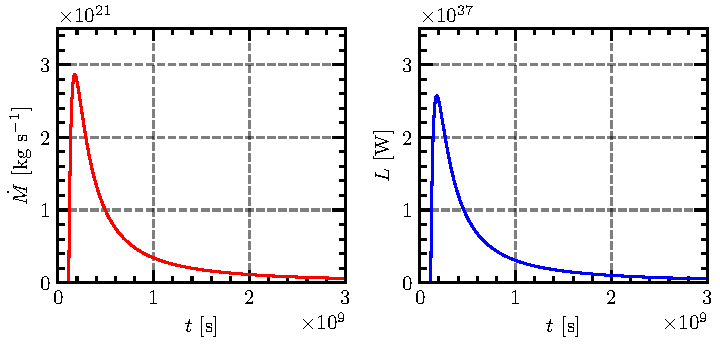
\includegraphics[width=5in]{images/mdot-lumens-metric.pdf}
			\caption{Left: Accretion rate in SI units. Right: Corresponding luminosity curve
			generated from the fallback rate.}
			\label{fig:mdot-lumens}
		\end{figure}

		Figure \ref{fig:mdot-lumens} shows the same event expressed in SI units. The left panel gives
		the mass fallback rate in $\mathrm{kg\,s^{-1}}$ as a function of time in seconds. The right
		panel shows the corresponding luminosity curve in watts, obtained using the accretion
		luminosity prescription $L=\eta\dot{M}c^2$, with a constant radiative efficiency $\eta=0.1$.
		Since $\eta$ and $c$ are constant, the luminosity is directly proportional to the fallback 
		rate, $L\propto\dot{M}$. Consequently, the luminosity curve has the same temporal dependence
		and overall shape as the mass fallback rate.
	
		Figure \ref{fig:mdot-mbh} shows the mass fallback rate of a $1 M_\odot$ star for black holes
		with masses ranging from $10^3 M_\odot$ to $10^8 M_\odot$. As in the previous calculations,
		the center-of-mass orbit is assumed to be parabolic, with $E_\star=0$ and $\delta=1$.
		The peak fallback time varies with black-hole mass because the characteristic return time of
		the debris depends on the energy spread induced by the tidal interaction. More massive black 
		holes produce a different characteristic fallback timescale, shifting the location of the peak
		in time. Despite this variation in the peak time and fallback rate, the late-time behavior of
		all cases approaches the same $T^{-5/3}$ power-law dependence predicted by the model.

		\newpage
		\begin{figure}[h!]
			\centering
			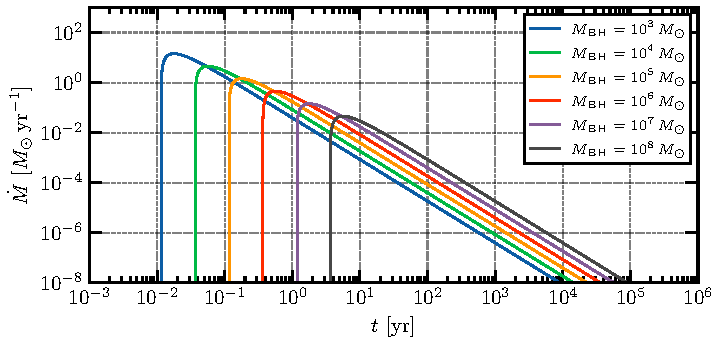
\includegraphics[width=5in]{images/mdot_mbh.pdf}
			\caption{Mass fallback rates for a $1 M_\odot$ star disrupted by black holes with masses 
			ranging from $10^3$ to $10^8 M_\odot$}
			\label{fig:mdot-mbh}
		\end{figure}

		Overall, we see from visual inspection that the mass fallback rate obtained under the 
		constant-density assumption closely resembles that obtained under a polytropic stellar model shown
		in the work of O\~na. In particular, both models exhibit an initial rise toward a peak fallback
		rate followed by a power-law decline at late times. This suggests that the constant-density model
		may provide a reasonable analytic approximation for capturing the general temporal behavior of
		the fallback rate.

		However, the apparent agreement between the two models is based only on the comparison of the 
		resulting curves and does not establish quantitative equivalence. The internal density profile of 
		a realistic star differs substantially from the constant-density assumption, particularly toward 
		the stellar center, and these differences can affect the distribution of debris orbital energies
		and consequently the detailed shape of the fallback curve. A more rigorous comparison would therefore 
		require numerical calculations using realistic stellar density profiles, such as polytropic or numerically
		evolved stellar models. Such simulations would allow the magnitude of the differences between the
		constant-density and polytropic results to be quantified and would determine the range over which
		the constant-density approximation remains valid.

	\newpage
	\section*{Appendices}
		\subsection*{Derivation of the tidal radius}
			From the potential $\Psi = -\dfrac{G\mbh}{r}$, we have
			\[
				\dv{\Psi(r-R_\star)}{r} = 
				\frac{G\mbh}{(r-R_\star)^2}  
			\]
			and
			\[
				\dv{\Psi(r+R_\star)}{r} = 
				\frac{G\mbh}{(r+R_\star)^2}  
			\]
			Therefore
			\[
				\frac{G\mbh}{(r-R_\star)^2}  
				-
				\frac{G\mbh}{(r+R_\star)^2}  
				=
				\frac{GM_\star}{R_\star^2} 
			\]
			We cancel $G$,
			\[
				\mbh \pqty{
				\frac{1}{(r-R_\star)^2}  
				-
				\frac{1}{(r+R_\star)^2}  
				}
				= 
				\frac{M_\star}{R_\star^2} 
			\]
			Evaluating the difference, we have
			\[
				\frac{1}{(r-R_\star)^2}
				-
				\frac{1}{(r+R_\star)^2}
				=
				\frac{4rR_\star}{(r^2 - R_\star^2)^2} 
			\]
			Hence
			\[
				\frac{4rR_\star}{(r^2 - R_\star^2)^2} 
				=
				\frac{M_\star}{R_\star^2} 
			\]
			Therefore
			\[
				(r^2-R_\star^2)^2 = 
				4 \frac{\mbh}{M_\star} r R_\star^3 
			\]
			For $r \gg R_\star$, since $(r^2-R_\star^2)^2 \simeq r^4$, we obtain
			\[
				r^4 \simeq
				4 \frac{\mbh}{M_\star} r R_\star^3 
			\]
			so
			\[
				r^3 \simeq
				4 \frac{\mbh}{M_\star} R_\star^3 
			\]
			Thus
			\[
				R_t \simeq
				\pqty{4 \frac{\mbh}{M_\star}}^{1/3} R_\star 
			\]
		\subsection*{Derivation of the mass element $dM$}
			For the star slices, we take the cylindrical slice at a distance $\Delta r$ from the center of the star. We introduce a variable $x$, which is 
			the radius of the cylinder at $\Delta r$. At the outer edge of the slice, $x$ is related to the sperical radius $r$ by
			\[
				x^2 = R_\star^2 - \Delta r^2
			\]

			To get the mass of the slice, and since the density is not uniform but is instead spherically symmetric, we approximate 
			it as a series of concentric rings with radius $x$, and height $\dd{\Delta r}$. We start from the center of the slice at 
			$x=0$, and at end at the edge of the star, at $x = \sqrt{R_\star^2 - (\Delta r)^2}$. The mass of the integrated cylinder 
			is therefore
			\[
				\dd{M} = 2\pi \dd{\Delta r} \int_0^{\sqrt{R_\star^2 - (\Delta r)^2}} \rho'(x) x \dd{x}
			\]
			where $\rho'$ is the density expressed as a funcion of the cylindrical radius $x$. Since the slice is located
			at a distance $\Delta r$ from the center, the cylindrical $x$ and the spherical radius $r$ are related by
			\[
				x^2 = r^2 - (\Delta r)^2
			\]
			Thus, the density function $\rho'(x)$ is related to the spherical density function $\rho(r)$ by
			\[
				\rho'(x) = \rho\qty(\sqrt{x^2 + (\Delta r)^2})
			\]
			To express the integral in terms of the spherical radius $r$, we differentiate $r^2 = x^2 + (\Delta r)^2$, where 
			$\Delta r$ is fixed for a given slice. We find that
			\[
				2r \dd{r} = 2x\dd{x}
			\]
			or
			\[
				x\dd{x} = r\dd{r}
			\]
			At the center of the slice, $x=0$, therefore $r = \Delta r$, and at the edge, $x = \sqrt{R_\star^2 - \Delta r^2}$, and hence, $r = R_\star$.
			We now subsitute $r\dd{r}$ in the integral and change the limits. We can also substitue in $\rho(r)$, the spherical density function. We now have
			the mass element of the slice in terms of the spherical radius
			\[
				\dd{M} = 2\pi \dd{\Delta r} \int_{\Delta r}^{R_\star} r \rho(r)  \dd{r}
			\]
	\label{appendices:a}	
	\bibliographystyle{unsrturl}
	\bibliography{references}
\end{document}
